% Created by tikzDevice version 0.12.3 on 2020-02-03 16:06:14
% !TEX encoding = UTF-8 Unicode
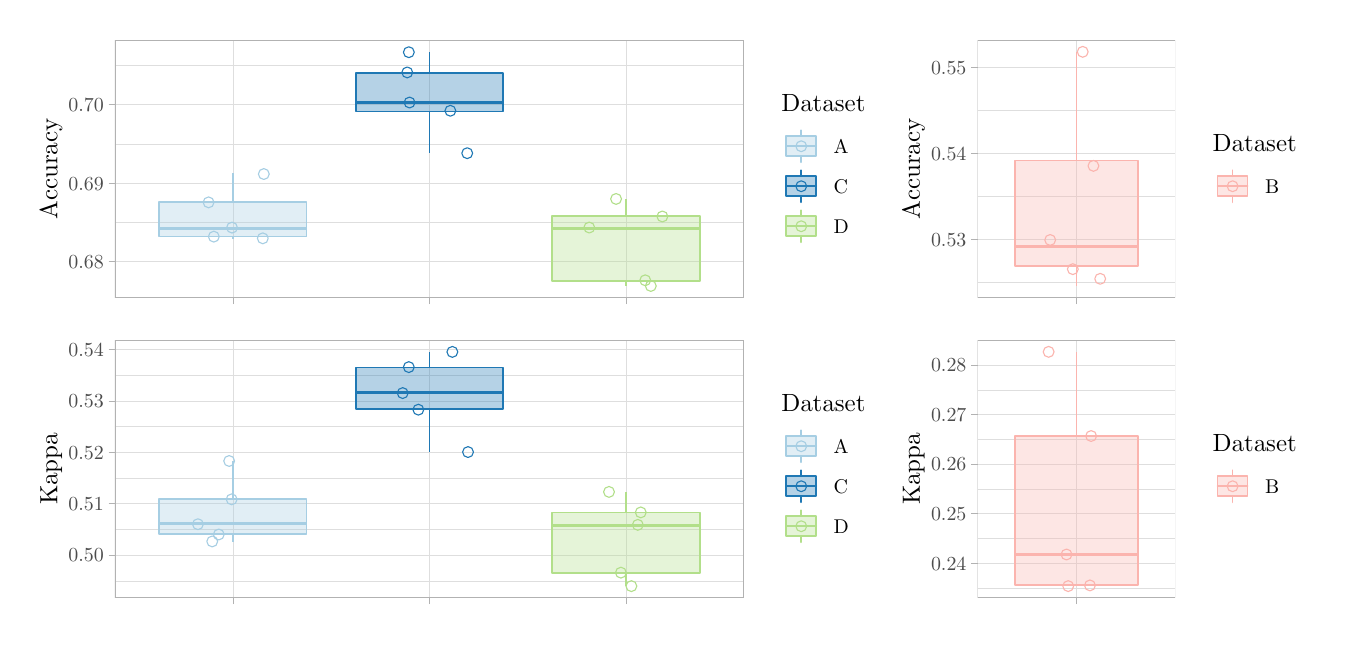
\begin{tikzpicture}[x=1pt,y=1pt]
\definecolor{fillColor}{RGB}{255,255,255}
\path[use as bounding box,fill=fillColor,fill opacity=0.00] (0,0) rectangle (467.59,216.81);
\begin{scope}
\path[clip] (  0.00,108.41) rectangle (311.72,216.81);
\definecolor{drawColor}{RGB}{255,255,255}
\definecolor{fillColor}{RGB}{255,255,255}

\path[draw=drawColor,line width= 0.5pt,line join=round,line cap=round,fill=fillColor] (  0.00,108.41) rectangle (311.72,216.81);
\end{scope}
\begin{scope}
\path[clip] ( 31.54,119.15) rectangle (258.81,212.31);
\definecolor{fillColor}{RGB}{255,255,255}

\path[fill=fillColor] ( 31.54,119.15) rectangle (258.81,212.31);
\definecolor{drawColor}{gray}{0.87}

\path[draw=drawColor,line width= 0.1pt,line join=round] ( 31.54,146.45) --
	(258.81,146.45);

\path[draw=drawColor,line width= 0.1pt,line join=round] ( 31.54,174.78) --
	(258.81,174.78);

\path[draw=drawColor,line width= 0.1pt,line join=round] ( 31.54,203.11) --
	(258.81,203.11);

\path[draw=drawColor,line width= 0.2pt,line join=round] ( 31.54,132.28) --
	(258.81,132.28);

\path[draw=drawColor,line width= 0.2pt,line join=round] ( 31.54,160.61) --
	(258.81,160.61);

\path[draw=drawColor,line width= 0.2pt,line join=round] ( 31.54,188.95) --
	(258.81,188.95);

\path[draw=drawColor,line width= 0.2pt,line join=round] ( 74.16,119.15) --
	( 74.16,212.31);

\path[draw=drawColor,line width= 0.2pt,line join=round] (145.18,119.15) --
	(145.18,212.31);

\path[draw=drawColor,line width= 0.2pt,line join=round] (216.20,119.15) --
	(216.20,212.31);
\definecolor{drawColor}{RGB}{166,206,227}

\path[draw=drawColor,line width= 0.6pt,line join=round] ( 74.16,153.81) -- ( 74.16,164.21);

\path[draw=drawColor,line width= 0.6pt,line join=round] ( 74.16,141.32) -- ( 74.16,140.46);
\definecolor{fillColor}{RGB}{166,206,227}

\path[draw=drawColor,line width= 0.6pt,line join=round,line cap=round,fill=fillColor,fill opacity=0.33] ( 47.52,153.81) --
	( 47.52,141.32) --
	(100.79,141.32) --
	(100.79,153.81) --
	( 47.52,153.81) --
	cycle;

\path[draw=drawColor,line width= 1.1pt,line join=round] ( 47.52,144.32) -- (100.79,144.32);
\definecolor{drawColor}{RGB}{31,120,180}

\path[draw=drawColor,line width= 0.6pt,line join=round] (145.18,200.43) -- (145.18,208.08);

\path[draw=drawColor,line width= 0.6pt,line join=round] (145.18,186.53) -- (145.18,171.43);
\definecolor{fillColor}{RGB}{31,120,180}

\path[draw=drawColor,line width= 0.6pt,line join=round,line cap=round,fill=fillColor,fill opacity=0.33] (118.54,200.43) --
	(118.54,186.53) --
	(171.81,186.53) --
	(171.81,200.43) --
	(118.54,200.43) --
	cycle;

\path[draw=drawColor,line width= 1.1pt,line join=round] (118.54,189.93) -- (171.81,189.93);
\definecolor{drawColor}{RGB}{178,223,138}

\path[draw=drawColor,line width= 0.6pt,line join=round] (216.20,148.74) -- (216.20,155.06);

\path[draw=drawColor,line width= 0.6pt,line join=round] (216.20,125.35) -- (216.20,123.39);
\definecolor{fillColor}{RGB}{178,223,138}

\path[draw=drawColor,line width= 0.6pt,line join=round,line cap=round,fill=fillColor,fill opacity=0.33] (189.56,148.74) --
	(189.56,125.35) --
	(242.83,125.35) --
	(242.83,148.74) --
	(189.56,148.74) --
	cycle;

\path[draw=drawColor,line width= 1.1pt,line join=round] (189.56,144.32) -- (242.83,144.32);
\definecolor{drawColor}{RGB}{166,206,227}

\path[draw=drawColor,line width= 0.4pt,line join=round,line cap=round] ( 65.37,153.68) circle (  1.96);

\path[draw=drawColor,line width= 0.4pt,line join=round,line cap=round] ( 84.96,140.69) circle (  1.96);

\path[draw=drawColor,line width= 0.4pt,line join=round,line cap=round] ( 67.26,141.30) circle (  1.96);

\path[draw=drawColor,line width= 0.4pt,line join=round,line cap=round] ( 73.84,144.56) circle (  1.96);

\path[draw=drawColor,line width= 0.4pt,line join=round,line cap=round] ( 85.33,163.92) circle (  1.96);
\definecolor{drawColor}{RGB}{31,120,180}

\path[draw=drawColor,line width= 0.4pt,line join=round,line cap=round] (137.73,207.94) circle (  1.96);

\path[draw=drawColor,line width= 0.4pt,line join=round,line cap=round] (137.99,189.76) circle (  1.96);

\path[draw=drawColor,line width= 0.4pt,line join=round,line cap=round] (158.83,171.45) circle (  1.96);

\path[draw=drawColor,line width= 0.4pt,line join=round,line cap=round] (137.16,200.63) circle (  1.96);

\path[draw=drawColor,line width= 0.4pt,line join=round,line cap=round] (152.74,186.78) circle (  1.96);
\definecolor{drawColor}{RGB}{178,223,138}

\path[draw=drawColor,line width= 0.4pt,line join=round,line cap=round] (229.35,148.58) circle (  1.96);

\path[draw=drawColor,line width= 0.4pt,line join=round,line cap=round] (212.62,154.92) circle (  1.96);

\path[draw=drawColor,line width= 0.4pt,line join=round,line cap=round] (225.17,123.47) circle (  1.96);

\path[draw=drawColor,line width= 0.4pt,line join=round,line cap=round] (202.93,144.58) circle (  1.96);

\path[draw=drawColor,line width= 0.4pt,line join=round,line cap=round] (223.16,125.53) circle (  1.96);
\definecolor{drawColor}{gray}{0.70}

\path[draw=drawColor,line width= 0.5pt,line join=round,line cap=round] ( 31.54,119.15) rectangle (258.81,212.31);
\end{scope}
\begin{scope}
\path[clip] (  0.00,  0.00) rectangle (467.59,216.81);
\definecolor{drawColor}{gray}{0.30}

\node[text=drawColor,anchor=base east,inner sep=0pt, outer sep=0pt, scale=  0.72] at ( 27.49,129.80) {0.68};

\node[text=drawColor,anchor=base east,inner sep=0pt, outer sep=0pt, scale=  0.72] at ( 27.49,158.13) {0.69};

\node[text=drawColor,anchor=base east,inner sep=0pt, outer sep=0pt, scale=  0.72] at ( 27.49,186.47) {0.70};
\end{scope}
\begin{scope}
\path[clip] (  0.00,  0.00) rectangle (467.59,216.81);
\definecolor{drawColor}{gray}{0.70}

\path[draw=drawColor,line width= 0.2pt,line join=round] ( 29.29,132.28) --
	( 31.54,132.28);

\path[draw=drawColor,line width= 0.2pt,line join=round] ( 29.29,160.61) --
	( 31.54,160.61);

\path[draw=drawColor,line width= 0.2pt,line join=round] ( 29.29,188.95) --
	( 31.54,188.95);
\end{scope}
\begin{scope}
\path[clip] (  0.00,  0.00) rectangle (467.59,216.81);
\definecolor{drawColor}{gray}{0.70}

\path[draw=drawColor,line width= 0.2pt,line join=round] ( 74.16,116.90) --
	( 74.16,119.15);

\path[draw=drawColor,line width= 0.2pt,line join=round] (145.18,116.90) --
	(145.18,119.15);

\path[draw=drawColor,line width= 0.2pt,line join=round] (216.20,116.90) --
	(216.20,119.15);
\end{scope}
\begin{scope}
\path[clip] (  0.00,  0.00) rectangle (467.59,216.81);
\definecolor{drawColor}{RGB}{0,0,0}

\node[text=drawColor,rotate= 90.00,anchor=base,inner sep=0pt, outer sep=0pt, scale=  0.90] at ( 10.70,165.73) {Accuracy};
\end{scope}
\begin{scope}
\path[clip] (  0.00,  0.00) rectangle (467.59,216.81);
\definecolor{fillColor}{RGB}{255,255,255}

\path[fill=fillColor] (267.81,133.33) rectangle (307.22,198.14);
\end{scope}
\begin{scope}
\path[clip] (  0.00,  0.00) rectangle (467.59,216.81);
\definecolor{drawColor}{RGB}{0,0,0}

\node[text=drawColor,anchor=base west,inner sep=0pt, outer sep=0pt, scale=  0.90] at (272.31,186.56) {Dataset};
\end{scope}
\begin{scope}
\path[clip] (  0.00,  0.00) rectangle (467.59,216.81);
\definecolor{fillColor}{RGB}{255,255,255}

\path[fill=fillColor] (272.31,166.74) rectangle (286.76,181.19);
\end{scope}
\begin{scope}
\path[clip] (  0.00,  0.00) rectangle (467.59,216.81);
\definecolor{drawColor}{RGB}{166,206,227}

\path[draw=drawColor,line width= 0.6pt,line join=round,line cap=round] (279.53,168.18) --
	(279.53,170.35);

\path[draw=drawColor,line width= 0.6pt,line join=round,line cap=round] (279.53,177.58) --
	(279.53,179.74);
\definecolor{fillColor}{RGB}{166,206,227}

\path[draw=drawColor,line width= 0.6pt,line join=round,line cap=round,fill=fillColor,fill opacity=0.33] (274.11,170.35) rectangle (284.95,177.58);

\path[draw=drawColor,line width= 0.6pt,line join=round,line cap=round] (274.11,173.96) --
	(284.95,173.96);
\end{scope}
\begin{scope}
\path[clip] (  0.00,  0.00) rectangle (467.59,216.81);
\definecolor{drawColor}{RGB}{166,206,227}

\path[draw=drawColor,line width= 0.4pt,line join=round,line cap=round] (279.53,173.96) circle (  1.96);
\end{scope}
\begin{scope}
\path[clip] (  0.00,  0.00) rectangle (467.59,216.81);
\definecolor{fillColor}{RGB}{255,255,255}

\path[fill=fillColor] (272.31,152.28) rectangle (286.76,166.74);
\end{scope}
\begin{scope}
\path[clip] (  0.00,  0.00) rectangle (467.59,216.81);
\definecolor{drawColor}{RGB}{31,120,180}

\path[draw=drawColor,line width= 0.6pt,line join=round,line cap=round] (279.53,153.73) --
	(279.53,155.89);

\path[draw=drawColor,line width= 0.6pt,line join=round,line cap=round] (279.53,163.12) --
	(279.53,165.29);
\definecolor{fillColor}{RGB}{31,120,180}

\path[draw=drawColor,line width= 0.6pt,line join=round,line cap=round,fill=fillColor,fill opacity=0.33] (274.11,155.89) rectangle (284.95,163.12);

\path[draw=drawColor,line width= 0.6pt,line join=round,line cap=round] (274.11,159.51) --
	(284.95,159.51);
\end{scope}
\begin{scope}
\path[clip] (  0.00,  0.00) rectangle (467.59,216.81);
\definecolor{drawColor}{RGB}{31,120,180}

\path[draw=drawColor,line width= 0.4pt,line join=round,line cap=round] (279.53,159.51) circle (  1.96);
\end{scope}
\begin{scope}
\path[clip] (  0.00,  0.00) rectangle (467.59,216.81);
\definecolor{fillColor}{RGB}{255,255,255}

\path[fill=fillColor] (272.31,137.83) rectangle (286.76,152.28);
\end{scope}
\begin{scope}
\path[clip] (  0.00,  0.00) rectangle (467.59,216.81);
\definecolor{drawColor}{RGB}{178,223,138}

\path[draw=drawColor,line width= 0.6pt,line join=round,line cap=round] (279.53,139.27) --
	(279.53,141.44);

\path[draw=drawColor,line width= 0.6pt,line join=round,line cap=round] (279.53,148.67) --
	(279.53,150.84);
\definecolor{fillColor}{RGB}{178,223,138}

\path[draw=drawColor,line width= 0.6pt,line join=round,line cap=round,fill=fillColor,fill opacity=0.33] (274.11,141.44) rectangle (284.95,148.67);

\path[draw=drawColor,line width= 0.6pt,line join=round,line cap=round] (274.11,145.05) --
	(284.95,145.05);
\end{scope}
\begin{scope}
\path[clip] (  0.00,  0.00) rectangle (467.59,216.81);
\definecolor{drawColor}{RGB}{178,223,138}

\path[draw=drawColor,line width= 0.4pt,line join=round,line cap=round] (279.53,145.05) circle (  1.96);
\end{scope}
\begin{scope}
\path[clip] (  0.00,  0.00) rectangle (467.59,216.81);
\definecolor{drawColor}{RGB}{0,0,0}

\node[text=drawColor,anchor=base west,inner sep=0pt, outer sep=0pt, scale=  0.72] at (291.26,171.48) {A};
\end{scope}
\begin{scope}
\path[clip] (  0.00,  0.00) rectangle (467.59,216.81);
\definecolor{drawColor}{RGB}{0,0,0}

\node[text=drawColor,anchor=base west,inner sep=0pt, outer sep=0pt, scale=  0.72] at (291.26,157.03) {C};
\end{scope}
\begin{scope}
\path[clip] (  0.00,  0.00) rectangle (467.59,216.81);
\definecolor{drawColor}{RGB}{0,0,0}

\node[text=drawColor,anchor=base west,inner sep=0pt, outer sep=0pt, scale=  0.72] at (291.26,142.57) {D};
\end{scope}
\begin{scope}
\path[clip] (311.72,108.41) rectangle (467.59,216.81);
\definecolor{drawColor}{RGB}{255,255,255}
\definecolor{fillColor}{RGB}{255,255,255}

\path[draw=drawColor,line width= 0.5pt,line join=round,line cap=round,fill=fillColor] (311.72,108.41) rectangle (467.59,216.81);
\end{scope}
\begin{scope}
\path[clip] (343.27,119.15) rectangle (414.67,212.31);
\definecolor{fillColor}{RGB}{255,255,255}

\path[fill=fillColor] (343.27,119.15) rectangle (414.67,212.31);
\definecolor{drawColor}{gray}{0.87}

\path[draw=drawColor,line width= 0.1pt,line join=round] (343.27,124.77) --
	(414.67,124.77);

\path[draw=drawColor,line width= 0.1pt,line join=round] (343.27,155.88) --
	(414.67,155.88);

\path[draw=drawColor,line width= 0.1pt,line join=round] (343.27,186.99) --
	(414.67,186.99);

\path[draw=drawColor,line width= 0.2pt,line join=round] (343.27,140.32) --
	(414.67,140.32);

\path[draw=drawColor,line width= 0.2pt,line join=round] (343.27,171.43) --
	(414.67,171.43);

\path[draw=drawColor,line width= 0.2pt,line join=round] (343.27,202.54) --
	(414.67,202.54);

\path[draw=drawColor,line width= 0.2pt,line join=round] (378.97,119.15) --
	(378.97,212.31);
\definecolor{drawColor}{RGB}{251,180,174}

\path[draw=drawColor,line width= 0.6pt,line join=round] (378.97,168.82) -- (378.97,207.92);

\path[draw=drawColor,line width= 0.6pt,line join=round] (378.97,130.64) -- (378.97,123.39);
\definecolor{fillColor}{RGB}{251,180,174}

\path[draw=drawColor,line width= 0.6pt,line join=round,line cap=round,fill=fillColor,fill opacity=0.33] (356.66,168.82) --
	(356.66,130.64) --
	(401.28,130.64) --
	(401.28,168.82) --
	(356.66,168.82) --
	cycle;

\path[draw=drawColor,line width= 1.1pt,line join=round] (356.66,137.63) -- (401.28,137.63);

\path[draw=drawColor,line width= 0.4pt,line join=round,line cap=round] (385.11,166.87) circle (  1.96);

\path[draw=drawColor,line width= 0.4pt,line join=round,line cap=round] (381.24,208.08) circle (  1.96);

\path[draw=drawColor,line width= 0.4pt,line join=round,line cap=round] (377.66,129.55) circle (  1.96);

\path[draw=drawColor,line width= 0.4pt,line join=round,line cap=round] (369.48,140.10) circle (  1.96);

\path[draw=drawColor,line width= 0.4pt,line join=round,line cap=round] (387.55,126.06) circle (  1.96);
\definecolor{drawColor}{gray}{0.70}

\path[draw=drawColor,line width= 0.5pt,line join=round,line cap=round] (343.27,119.15) rectangle (414.67,212.31);
\end{scope}
\begin{scope}
\path[clip] (  0.00,  0.00) rectangle (467.59,216.81);
\definecolor{drawColor}{gray}{0.30}

\node[text=drawColor,anchor=base east,inner sep=0pt, outer sep=0pt, scale=  0.72] at (339.22,137.84) {0.53};

\node[text=drawColor,anchor=base east,inner sep=0pt, outer sep=0pt, scale=  0.72] at (339.22,168.95) {0.54};

\node[text=drawColor,anchor=base east,inner sep=0pt, outer sep=0pt, scale=  0.72] at (339.22,200.06) {0.55};
\end{scope}
\begin{scope}
\path[clip] (  0.00,  0.00) rectangle (467.59,216.81);
\definecolor{drawColor}{gray}{0.70}

\path[draw=drawColor,line width= 0.2pt,line join=round] (341.02,140.32) --
	(343.27,140.32);

\path[draw=drawColor,line width= 0.2pt,line join=round] (341.02,171.43) --
	(343.27,171.43);

\path[draw=drawColor,line width= 0.2pt,line join=round] (341.02,202.54) --
	(343.27,202.54);
\end{scope}
\begin{scope}
\path[clip] (  0.00,  0.00) rectangle (467.59,216.81);
\definecolor{drawColor}{gray}{0.70}

\path[draw=drawColor,line width= 0.2pt,line join=round] (378.97,116.90) --
	(378.97,119.15);
\end{scope}
\begin{scope}
\path[clip] (  0.00,  0.00) rectangle (467.59,216.81);
\definecolor{drawColor}{RGB}{0,0,0}

\node[text=drawColor,rotate= 90.00,anchor=base,inner sep=0pt, outer sep=0pt, scale=  0.90] at (322.42,165.73) {Accuracy};
\end{scope}
\begin{scope}
\path[clip] (  0.00,  0.00) rectangle (467.59,216.81);
\definecolor{fillColor}{RGB}{255,255,255}

\path[fill=fillColor] (423.67,147.78) rectangle (463.09,183.68);
\end{scope}
\begin{scope}
\path[clip] (  0.00,  0.00) rectangle (467.59,216.81);
\definecolor{drawColor}{RGB}{0,0,0}

\node[text=drawColor,anchor=base west,inner sep=0pt, outer sep=0pt, scale=  0.90] at (428.17,172.11) {Dataset};
\end{scope}
\begin{scope}
\path[clip] (  0.00,  0.00) rectangle (467.59,216.81);
\definecolor{fillColor}{RGB}{255,255,255}

\path[fill=fillColor] (428.17,152.28) rectangle (442.62,166.74);
\end{scope}
\begin{scope}
\path[clip] (  0.00,  0.00) rectangle (467.59,216.81);
\definecolor{drawColor}{RGB}{251,180,174}

\path[draw=drawColor,line width= 0.6pt,line join=round,line cap=round] (435.40,153.73) --
	(435.40,155.89);

\path[draw=drawColor,line width= 0.6pt,line join=round,line cap=round] (435.40,163.12) --
	(435.40,165.29);
\definecolor{fillColor}{RGB}{251,180,174}

\path[draw=drawColor,line width= 0.6pt,line join=round,line cap=round,fill=fillColor,fill opacity=0.33] (429.98,155.89) rectangle (440.82,163.12);

\path[draw=drawColor,line width= 0.6pt,line join=round,line cap=round] (429.98,159.51) --
	(440.82,159.51);
\end{scope}
\begin{scope}
\path[clip] (  0.00,  0.00) rectangle (467.59,216.81);
\definecolor{drawColor}{RGB}{251,180,174}

\path[draw=drawColor,line width= 0.4pt,line join=round,line cap=round] (435.40,159.51) circle (  1.96);
\end{scope}
\begin{scope}
\path[clip] (  0.00,  0.00) rectangle (467.59,216.81);
\definecolor{drawColor}{RGB}{0,0,0}

\node[text=drawColor,anchor=base west,inner sep=0pt, outer sep=0pt, scale=  0.72] at (447.12,157.03) {B};
\end{scope}
\begin{scope}
\path[clip] (  0.00,  0.00) rectangle (311.72,108.41);
\definecolor{drawColor}{RGB}{255,255,255}
\definecolor{fillColor}{RGB}{255,255,255}

\path[draw=drawColor,line width= 0.5pt,line join=round,line cap=round,fill=fillColor] (  0.00,  0.00) rectangle (311.72,108.41);
\end{scope}
\begin{scope}
\path[clip] ( 31.54, 10.75) rectangle (258.81,103.91);
\definecolor{fillColor}{RGB}{255,255,255}

\path[fill=fillColor] ( 31.54, 10.75) rectangle (258.81,103.90);
\definecolor{drawColor}{gray}{0.87}

\path[draw=drawColor,line width= 0.1pt,line join=round] ( 31.54, 16.99) --
	(258.81, 16.99);

\path[draw=drawColor,line width= 0.1pt,line join=round] ( 31.54, 35.55) --
	(258.81, 35.55);

\path[draw=drawColor,line width= 0.1pt,line join=round] ( 31.54, 54.11) --
	(258.81, 54.11);

\path[draw=drawColor,line width= 0.1pt,line join=round] ( 31.54, 72.66) --
	(258.81, 72.66);

\path[draw=drawColor,line width= 0.1pt,line join=round] ( 31.54, 91.22) --
	(258.81, 91.22);

\path[draw=drawColor,line width= 0.2pt,line join=round] ( 31.54, 26.27) --
	(258.81, 26.27);

\path[draw=drawColor,line width= 0.2pt,line join=round] ( 31.54, 44.83) --
	(258.81, 44.83);

\path[draw=drawColor,line width= 0.2pt,line join=round] ( 31.54, 63.39) --
	(258.81, 63.39);

\path[draw=drawColor,line width= 0.2pt,line join=round] ( 31.54, 81.94) --
	(258.81, 81.94);

\path[draw=drawColor,line width= 0.2pt,line join=round] ( 31.54,100.50) --
	(258.81,100.50);

\path[draw=drawColor,line width= 0.2pt,line join=round] ( 74.16, 10.75) --
	( 74.16,103.91);

\path[draw=drawColor,line width= 0.2pt,line join=round] (145.18, 10.75) --
	(145.18,103.91);

\path[draw=drawColor,line width= 0.2pt,line join=round] (216.20, 10.75) --
	(216.20,103.91);
\definecolor{drawColor}{RGB}{166,206,227}

\path[draw=drawColor,line width= 0.6pt,line join=round] ( 74.16, 46.52) -- ( 74.16, 60.09);

\path[draw=drawColor,line width= 0.6pt,line join=round] ( 74.16, 33.78) -- ( 74.16, 30.99);
\definecolor{fillColor}{RGB}{166,206,227}

\path[draw=drawColor,line width= 0.6pt,line join=round,line cap=round,fill=fillColor,fill opacity=0.33] ( 47.52, 46.52) --
	( 47.52, 33.78) --
	(100.79, 33.78) --
	(100.79, 46.52) --
	( 47.52, 46.52) --
	cycle;

\path[draw=drawColor,line width= 1.1pt,line join=round] ( 47.52, 37.52) -- (100.79, 37.52);
\definecolor{drawColor}{RGB}{31,120,180}

\path[draw=drawColor,line width= 0.6pt,line join=round] (145.18, 94.00) -- (145.18, 99.67);

\path[draw=drawColor,line width= 0.6pt,line join=round] (145.18, 78.93) -- (145.18, 63.56);
\definecolor{fillColor}{RGB}{31,120,180}

\path[draw=drawColor,line width= 0.6pt,line join=round,line cap=round,fill=fillColor,fill opacity=0.33] (118.54, 94.00) --
	(118.54, 78.93) --
	(171.81, 78.93) --
	(171.81, 94.00) --
	(118.54, 94.00) --
	cycle;

\path[draw=drawColor,line width= 1.1pt,line join=round] (118.54, 84.92) -- (171.81, 84.92);
\definecolor{drawColor}{RGB}{178,223,138}

\path[draw=drawColor,line width= 0.6pt,line join=round] (216.20, 41.58) -- (216.20, 49.01);

\path[draw=drawColor,line width= 0.6pt,line join=round] (216.20, 19.87) -- (216.20, 14.98);
\definecolor{fillColor}{RGB}{178,223,138}

\path[draw=drawColor,line width= 0.6pt,line join=round,line cap=round,fill=fillColor,fill opacity=0.33] (189.56, 41.58) --
	(189.56, 19.87) --
	(242.83, 19.87) --
	(242.83, 41.58) --
	(189.56, 41.58) --
	cycle;

\path[draw=drawColor,line width= 1.1pt,line join=round] (189.56, 37.08) -- (242.83, 37.08);
\definecolor{drawColor}{RGB}{166,206,227}

\path[draw=drawColor,line width= 0.4pt,line join=round,line cap=round] ( 73.71, 46.37) circle (  1.96);

\path[draw=drawColor,line width= 0.4pt,line join=round,line cap=round] ( 66.69, 31.16) circle (  1.96);

\path[draw=drawColor,line width= 0.4pt,line join=round,line cap=round] ( 69.05, 33.67) circle (  1.96);

\path[draw=drawColor,line width= 0.4pt,line join=round,line cap=round] ( 61.52, 37.39) circle (  1.96);

\path[draw=drawColor,line width= 0.4pt,line join=round,line cap=round] ( 72.81, 60.23) circle (  1.96);
\definecolor{drawColor}{RGB}{31,120,180}

\path[draw=drawColor,line width= 0.4pt,line join=round,line cap=round] (153.46, 99.65) circle (  1.96);

\path[draw=drawColor,line width= 0.4pt,line join=round,line cap=round] (135.51, 84.77) circle (  1.96);

\path[draw=drawColor,line width= 0.4pt,line join=round,line cap=round] (159.12, 63.46) circle (  1.96);

\path[draw=drawColor,line width= 0.4pt,line join=round,line cap=round] (137.72, 94.15) circle (  1.96);

\path[draw=drawColor,line width= 0.4pt,line join=round,line cap=round] (141.17, 78.77) circle (  1.96);
\definecolor{drawColor}{RGB}{178,223,138}

\path[draw=drawColor,line width= 0.4pt,line join=round,line cap=round] (221.54, 41.65) circle (  1.96);

\path[draw=drawColor,line width= 0.4pt,line join=round,line cap=round] (210.06, 49.06) circle (  1.96);

\path[draw=drawColor,line width= 0.4pt,line join=round,line cap=round] (218.15, 15.01) circle (  1.96);

\path[draw=drawColor,line width= 0.4pt,line join=round,line cap=round] (220.47, 37.15) circle (  1.96);

\path[draw=drawColor,line width= 0.4pt,line join=round,line cap=round] (214.36, 19.88) circle (  1.96);
\definecolor{drawColor}{gray}{0.70}

\path[draw=drawColor,line width= 0.5pt,line join=round,line cap=round] ( 31.54, 10.75) rectangle (258.81,103.90);
\end{scope}
\begin{scope}
\path[clip] (  0.00,  0.00) rectangle (467.59,216.81);
\definecolor{drawColor}{gray}{0.30}

\node[text=drawColor,anchor=base east,inner sep=0pt, outer sep=0pt, scale=  0.72] at ( 27.49, 23.79) {0.50};

\node[text=drawColor,anchor=base east,inner sep=0pt, outer sep=0pt, scale=  0.72] at ( 27.49, 42.35) {0.51};

\node[text=drawColor,anchor=base east,inner sep=0pt, outer sep=0pt, scale=  0.72] at ( 27.49, 60.91) {0.52};

\node[text=drawColor,anchor=base east,inner sep=0pt, outer sep=0pt, scale=  0.72] at ( 27.49, 79.46) {0.53};

\node[text=drawColor,anchor=base east,inner sep=0pt, outer sep=0pt, scale=  0.72] at ( 27.49, 98.02) {0.54};
\end{scope}
\begin{scope}
\path[clip] (  0.00,  0.00) rectangle (467.59,216.81);
\definecolor{drawColor}{gray}{0.70}

\path[draw=drawColor,line width= 0.2pt,line join=round] ( 29.29, 26.27) --
	( 31.54, 26.27);

\path[draw=drawColor,line width= 0.2pt,line join=round] ( 29.29, 44.83) --
	( 31.54, 44.83);

\path[draw=drawColor,line width= 0.2pt,line join=round] ( 29.29, 63.39) --
	( 31.54, 63.39);

\path[draw=drawColor,line width= 0.2pt,line join=round] ( 29.29, 81.94) --
	( 31.54, 81.94);

\path[draw=drawColor,line width= 0.2pt,line join=round] ( 29.29,100.50) --
	( 31.54,100.50);
\end{scope}
\begin{scope}
\path[clip] (  0.00,  0.00) rectangle (467.59,216.81);
\definecolor{drawColor}{gray}{0.70}

\path[draw=drawColor,line width= 0.2pt,line join=round] ( 74.16,  8.50) --
	( 74.16, 10.75);

\path[draw=drawColor,line width= 0.2pt,line join=round] (145.18,  8.50) --
	(145.18, 10.75);

\path[draw=drawColor,line width= 0.2pt,line join=round] (216.20,  8.50) --
	(216.20, 10.75);
\end{scope}
\begin{scope}
\path[clip] (  0.00,  0.00) rectangle (467.59,216.81);
\definecolor{drawColor}{RGB}{0,0,0}

\node[text=drawColor,rotate= 90.00,anchor=base,inner sep=0pt, outer sep=0pt, scale=  0.90] at ( 10.70, 57.33) {Kappa};
\end{scope}
\begin{scope}
\path[clip] (  0.00,  0.00) rectangle (467.59,216.81);
\definecolor{fillColor}{RGB}{255,255,255}

\path[fill=fillColor] (267.81, 24.92) rectangle (307.22, 89.73);
\end{scope}
\begin{scope}
\path[clip] (  0.00,  0.00) rectangle (467.59,216.81);
\definecolor{drawColor}{RGB}{0,0,0}

\node[text=drawColor,anchor=base west,inner sep=0pt, outer sep=0pt, scale=  0.90] at (272.31, 78.16) {Dataset};
\end{scope}
\begin{scope}
\path[clip] (  0.00,  0.00) rectangle (467.59,216.81);
\definecolor{fillColor}{RGB}{255,255,255}

\path[fill=fillColor] (272.31, 58.33) rectangle (286.76, 72.78);
\end{scope}
\begin{scope}
\path[clip] (  0.00,  0.00) rectangle (467.59,216.81);
\definecolor{drawColor}{RGB}{166,206,227}

\path[draw=drawColor,line width= 0.6pt,line join=round,line cap=round] (279.53, 59.78) --
	(279.53, 61.94);

\path[draw=drawColor,line width= 0.6pt,line join=round,line cap=round] (279.53, 69.17) --
	(279.53, 71.34);
\definecolor{fillColor}{RGB}{166,206,227}

\path[draw=drawColor,line width= 0.6pt,line join=round,line cap=round,fill=fillColor,fill opacity=0.33] (274.11, 61.94) rectangle (284.95, 69.17);

\path[draw=drawColor,line width= 0.6pt,line join=round,line cap=round] (274.11, 65.56) --
	(284.95, 65.56);
\end{scope}
\begin{scope}
\path[clip] (  0.00,  0.00) rectangle (467.59,216.81);
\definecolor{drawColor}{RGB}{166,206,227}

\path[draw=drawColor,line width= 0.4pt,line join=round,line cap=round] (279.53, 65.56) circle (  1.96);
\end{scope}
\begin{scope}
\path[clip] (  0.00,  0.00) rectangle (467.59,216.81);
\definecolor{fillColor}{RGB}{255,255,255}

\path[fill=fillColor] (272.31, 43.88) rectangle (286.76, 58.33);
\end{scope}
\begin{scope}
\path[clip] (  0.00,  0.00) rectangle (467.59,216.81);
\definecolor{drawColor}{RGB}{31,120,180}

\path[draw=drawColor,line width= 0.6pt,line join=round,line cap=round] (279.53, 45.32) --
	(279.53, 47.49);

\path[draw=drawColor,line width= 0.6pt,line join=round,line cap=round] (279.53, 54.72) --
	(279.53, 56.88);
\definecolor{fillColor}{RGB}{31,120,180}

\path[draw=drawColor,line width= 0.6pt,line join=round,line cap=round,fill=fillColor,fill opacity=0.33] (274.11, 47.49) rectangle (284.95, 54.72);

\path[draw=drawColor,line width= 0.6pt,line join=round,line cap=round] (274.11, 51.10) --
	(284.95, 51.10);
\end{scope}
\begin{scope}
\path[clip] (  0.00,  0.00) rectangle (467.59,216.81);
\definecolor{drawColor}{RGB}{31,120,180}

\path[draw=drawColor,line width= 0.4pt,line join=round,line cap=round] (279.53, 51.10) circle (  1.96);
\end{scope}
\begin{scope}
\path[clip] (  0.00,  0.00) rectangle (467.59,216.81);
\definecolor{fillColor}{RGB}{255,255,255}

\path[fill=fillColor] (272.31, 29.42) rectangle (286.76, 43.88);
\end{scope}
\begin{scope}
\path[clip] (  0.00,  0.00) rectangle (467.59,216.81);
\definecolor{drawColor}{RGB}{178,223,138}

\path[draw=drawColor,line width= 0.6pt,line join=round,line cap=round] (279.53, 30.87) --
	(279.53, 33.04);

\path[draw=drawColor,line width= 0.6pt,line join=round,line cap=round] (279.53, 40.26) --
	(279.53, 42.43);
\definecolor{fillColor}{RGB}{178,223,138}

\path[draw=drawColor,line width= 0.6pt,line join=round,line cap=round,fill=fillColor,fill opacity=0.33] (274.11, 33.04) rectangle (284.95, 40.26);

\path[draw=drawColor,line width= 0.6pt,line join=round,line cap=round] (274.11, 36.65) --
	(284.95, 36.65);
\end{scope}
\begin{scope}
\path[clip] (  0.00,  0.00) rectangle (467.59,216.81);
\definecolor{drawColor}{RGB}{178,223,138}

\path[draw=drawColor,line width= 0.4pt,line join=round,line cap=round] (279.53, 36.65) circle (  1.96);
\end{scope}
\begin{scope}
\path[clip] (  0.00,  0.00) rectangle (467.59,216.81);
\definecolor{drawColor}{RGB}{0,0,0}

\node[text=drawColor,anchor=base west,inner sep=0pt, outer sep=0pt, scale=  0.72] at (291.26, 63.08) {A};
\end{scope}
\begin{scope}
\path[clip] (  0.00,  0.00) rectangle (467.59,216.81);
\definecolor{drawColor}{RGB}{0,0,0}

\node[text=drawColor,anchor=base west,inner sep=0pt, outer sep=0pt, scale=  0.72] at (291.26, 48.62) {C};
\end{scope}
\begin{scope}
\path[clip] (  0.00,  0.00) rectangle (467.59,216.81);
\definecolor{drawColor}{RGB}{0,0,0}

\node[text=drawColor,anchor=base west,inner sep=0pt, outer sep=0pt, scale=  0.72] at (291.26, 34.17) {D};
\end{scope}
\begin{scope}
\path[clip] (311.72,  0.00) rectangle (467.59,108.41);
\definecolor{drawColor}{RGB}{255,255,255}
\definecolor{fillColor}{RGB}{255,255,255}

\path[draw=drawColor,line width= 0.5pt,line join=round,line cap=round,fill=fillColor] (311.72,  0.00) rectangle (467.59,108.41);
\end{scope}
\begin{scope}
\path[clip] (343.27, 10.75) rectangle (414.67,103.91);
\definecolor{fillColor}{RGB}{255,255,255}

\path[fill=fillColor] (343.27, 10.75) rectangle (414.67,103.90);
\definecolor{drawColor}{gray}{0.87}

\path[draw=drawColor,line width= 0.1pt,line join=round] (343.27, 14.37) --
	(414.67, 14.37);

\path[draw=drawColor,line width= 0.1pt,line join=round] (343.27, 32.26) --
	(414.67, 32.26);

\path[draw=drawColor,line width= 0.1pt,line join=round] (343.27, 50.16) --
	(414.67, 50.16);

\path[draw=drawColor,line width= 0.1pt,line join=round] (343.27, 68.06) --
	(414.67, 68.06);

\path[draw=drawColor,line width= 0.1pt,line join=round] (343.27, 85.95) --
	(414.67, 85.95);

\path[draw=drawColor,line width= 0.1pt,line join=round] (343.27,103.85) --
	(414.67,103.85);

\path[draw=drawColor,line width= 0.2pt,line join=round] (343.27, 23.32) --
	(414.67, 23.32);

\path[draw=drawColor,line width= 0.2pt,line join=round] (343.27, 41.21) --
	(414.67, 41.21);

\path[draw=drawColor,line width= 0.2pt,line join=round] (343.27, 59.11) --
	(414.67, 59.11);

\path[draw=drawColor,line width= 0.2pt,line join=round] (343.27, 77.01) --
	(414.67, 77.01);

\path[draw=drawColor,line width= 0.2pt,line join=round] (343.27, 94.90) --
	(414.67, 94.90);

\path[draw=drawColor,line width= 0.2pt,line join=round] (378.97, 10.75) --
	(378.97,103.91);
\definecolor{drawColor}{RGB}{251,180,174}

\path[draw=drawColor,line width= 0.6pt,line join=round] (378.97, 69.32) -- (378.97, 99.54);

\path[draw=drawColor,line width= 0.6pt,line join=round] (378.97, 15.34) -- (378.97, 14.98);
\definecolor{fillColor}{RGB}{251,180,174}

\path[draw=drawColor,line width= 0.6pt,line join=round,line cap=round,fill=fillColor,fill opacity=0.33] (356.66, 69.32) --
	(356.66, 15.34) --
	(401.28, 15.34) --
	(401.28, 69.32) --
	(356.66, 69.32) --
	cycle;

\path[draw=drawColor,line width= 1.1pt,line join=round] (356.66, 26.45) -- (401.28, 26.45);

\path[draw=drawColor,line width= 0.4pt,line join=round,line cap=round] (384.28, 69.25) circle (  1.96);

\path[draw=drawColor,line width= 0.4pt,line join=round,line cap=round] (368.92, 99.67) circle (  1.96);

\path[draw=drawColor,line width= 0.4pt,line join=round,line cap=round] (375.38, 26.44) circle (  1.96);

\path[draw=drawColor,line width= 0.4pt,line join=round,line cap=round] (383.85, 15.27) circle (  1.96);

\path[draw=drawColor,line width= 0.4pt,line join=round,line cap=round] (375.99, 15.02) circle (  1.96);
\definecolor{drawColor}{gray}{0.70}

\path[draw=drawColor,line width= 0.5pt,line join=round,line cap=round] (343.27, 10.75) rectangle (414.67,103.90);
\end{scope}
\begin{scope}
\path[clip] (  0.00,  0.00) rectangle (467.59,216.81);
\definecolor{drawColor}{gray}{0.30}

\node[text=drawColor,anchor=base east,inner sep=0pt, outer sep=0pt, scale=  0.72] at (339.22, 20.84) {0.24};

\node[text=drawColor,anchor=base east,inner sep=0pt, outer sep=0pt, scale=  0.72] at (339.22, 38.73) {0.25};

\node[text=drawColor,anchor=base east,inner sep=0pt, outer sep=0pt, scale=  0.72] at (339.22, 56.63) {0.26};

\node[text=drawColor,anchor=base east,inner sep=0pt, outer sep=0pt, scale=  0.72] at (339.22, 74.53) {0.27};

\node[text=drawColor,anchor=base east,inner sep=0pt, outer sep=0pt, scale=  0.72] at (339.22, 92.42) {0.28};
\end{scope}
\begin{scope}
\path[clip] (  0.00,  0.00) rectangle (467.59,216.81);
\definecolor{drawColor}{gray}{0.70}

\path[draw=drawColor,line width= 0.2pt,line join=round] (341.02, 23.32) --
	(343.27, 23.32);

\path[draw=drawColor,line width= 0.2pt,line join=round] (341.02, 41.21) --
	(343.27, 41.21);

\path[draw=drawColor,line width= 0.2pt,line join=round] (341.02, 59.11) --
	(343.27, 59.11);

\path[draw=drawColor,line width= 0.2pt,line join=round] (341.02, 77.01) --
	(343.27, 77.01);

\path[draw=drawColor,line width= 0.2pt,line join=round] (341.02, 94.90) --
	(343.27, 94.90);
\end{scope}
\begin{scope}
\path[clip] (  0.00,  0.00) rectangle (467.59,216.81);
\definecolor{drawColor}{gray}{0.70}

\path[draw=drawColor,line width= 0.2pt,line join=round] (378.97,  8.50) --
	(378.97, 10.75);
\end{scope}
\begin{scope}
\path[clip] (  0.00,  0.00) rectangle (467.59,216.81);
\definecolor{drawColor}{RGB}{0,0,0}

\node[text=drawColor,rotate= 90.00,anchor=base,inner sep=0pt, outer sep=0pt, scale=  0.90] at (322.42, 57.33) {Kappa};
\end{scope}
\begin{scope}
\path[clip] (  0.00,  0.00) rectangle (467.59,216.81);
\definecolor{fillColor}{RGB}{255,255,255}

\path[fill=fillColor] (423.67, 39.38) rectangle (463.09, 75.28);
\end{scope}
\begin{scope}
\path[clip] (  0.00,  0.00) rectangle (467.59,216.81);
\definecolor{drawColor}{RGB}{0,0,0}

\node[text=drawColor,anchor=base west,inner sep=0pt, outer sep=0pt, scale=  0.90] at (428.17, 63.71) {Dataset};
\end{scope}
\begin{scope}
\path[clip] (  0.00,  0.00) rectangle (467.59,216.81);
\definecolor{fillColor}{RGB}{255,255,255}

\path[fill=fillColor] (428.17, 43.88) rectangle (442.62, 58.33);
\end{scope}
\begin{scope}
\path[clip] (  0.00,  0.00) rectangle (467.59,216.81);
\definecolor{drawColor}{RGB}{251,180,174}

\path[draw=drawColor,line width= 0.6pt,line join=round,line cap=round] (435.40, 45.32) --
	(435.40, 47.49);

\path[draw=drawColor,line width= 0.6pt,line join=round,line cap=round] (435.40, 54.72) --
	(435.40, 56.88);
\definecolor{fillColor}{RGB}{251,180,174}

\path[draw=drawColor,line width= 0.6pt,line join=round,line cap=round,fill=fillColor,fill opacity=0.33] (429.98, 47.49) rectangle (440.82, 54.72);

\path[draw=drawColor,line width= 0.6pt,line join=round,line cap=round] (429.98, 51.10) --
	(440.82, 51.10);
\end{scope}
\begin{scope}
\path[clip] (  0.00,  0.00) rectangle (467.59,216.81);
\definecolor{drawColor}{RGB}{251,180,174}

\path[draw=drawColor,line width= 0.4pt,line join=round,line cap=round] (435.40, 51.10) circle (  1.96);
\end{scope}
\begin{scope}
\path[clip] (  0.00,  0.00) rectangle (467.59,216.81);
\definecolor{drawColor}{RGB}{0,0,0}

\node[text=drawColor,anchor=base west,inner sep=0pt, outer sep=0pt, scale=  0.72] at (447.12, 48.62) {B};
\end{scope}
\end{tikzpicture}
